% Terzaghi consolidation, plane-strain rectangle: loading and boundary conditions.
% Build: pdflatex terzaghi_plane_strain.tex && pdftocairo -svg terzaghi_plane_strain.pdf terzaghi_plane_strain.svg
\documentclass[tikz,border=4pt]{standalone}
\usetikzlibrary{arrows.meta,patterns,calc}
\tikzset{
	load/.style={-{Latex[length=2mm]},thick,red!70!black},
	dim/.style={{Latex[length=2mm]}-{Latex[length=2mm]},thin},
	roller/.style={draw,thick,fill=white,circle,inner sep=0pt,minimum size=2.2mm},
}
\begin{document}
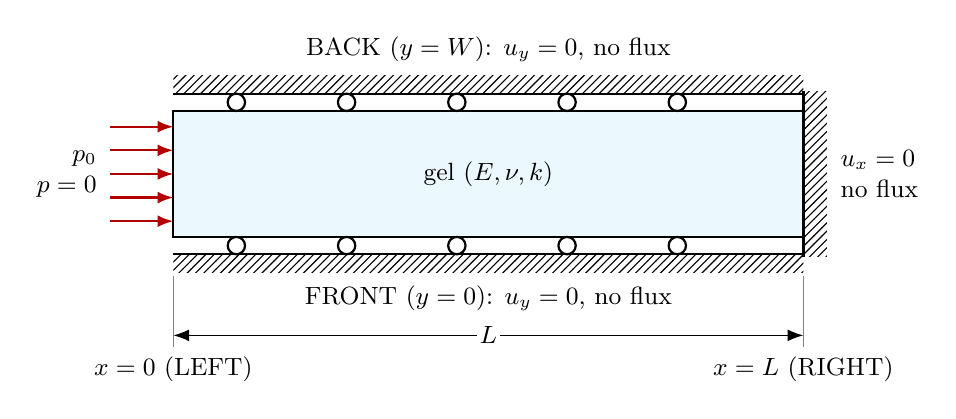
\begin{tikzpicture}[font=\small]
	\def\L{8} \def\H{1.6}
	\draw[thick,fill=cyan!8] (0,0) rectangle (\L,\H);
	\node at (\L/2,\H/2) {gel $(E, \nu, k)$};
	% RIGHT x = L
	\fill[pattern=north east lines] (\L,-0.25) rectangle (\L+0.3,\H+0.25);
	\draw[very thick] (\L,-0.25) -- (\L,\H+0.25);
	\node[right,align=left] at (\L+0.35,\H/2) {$u_x = 0$\\ no flux};
	% LEFT x = 0
	\foreach \y in {0.2,0.5,...,1.45} \draw[load] (-0.8,\y) -- (0,\y);
	\node[left,align=right] at (-0.85,\H/2) {$p_0$\\ $p = 0$};
	% FRONT / BACK: rollers
	\foreach \x in {0.8,2.2,...,7.5} {\node[roller] at (\x,-0.11) {}; \node[roller] at (\x,\H+0.11) {};}
	\fill[pattern=north east lines] (0,-0.22) rectangle (\L,-0.45); \draw[thick] (0,-0.22) -- (\L,-0.22);
	\fill[pattern=north east lines] (0,\H+0.22) rectangle (\L,\H+0.45); \draw[thick] (0,\H+0.22) -- (\L,\H+0.22);
	\node[below] at (\L/2,-0.5) {FRONT $(y = 0)$: $u_y = 0$, no flux};
	\node[above] at (\L/2,\H+0.5) {BACK $(y = W)$: $u_y = 0$, no flux};
	% dimensions
	\draw[dim] (0,-1.25) -- node[fill=white,inner sep=1pt] {$L$} (\L,-1.25);
	\draw[thin,gray] (0,-0.5) -- (0,-1.4) (\L,-0.5) -- (\L,-1.4);
	\node[below] at (0,-1.4) {$x = 0$ (LEFT)};
	\node[below] at (\L,-1.4) {$x = L$ (RIGHT)};
\end{tikzpicture}
\end{document}
